\graphicspath{{chapters/05/}}
\chapter{Approximation methods}
How do we solve quantum mechanical problems? Or to be more specific, how to solve the (stationary) Schrodinger equation $ H \psi = E \psi$? There are some "solvable" problems, for which we get a wave function to fit any desired value.
As the problems become more complicated, even by relying on super computers it is impossible to design algorithms that provide for an exact solution.
Here's the need for approximation methods.
Approximation methods can be "ideal" and "non-ideal" (not conventional names).
An ideal approximation method can become an exact method by tuning some parameters, the non-ideal ones will always remain an approximation, even with huge computational power (many in biology are non-ideal, like the Hartree-Fock, and are developed upon a physical intuition that allows to make important assumptions).
Some assumption concern the shape of the Hamiltonian (like confining a particle in a box instead of a complex potential), some concern the solution of a given Hamiltonian.
The question we ask ourselves as biologist is "do we want to be more accurate or insightful?".
If our aim is a biological application of quantum mechanics we are more interested in accuracy rather than completely understanding a structure $\rightarrow$ approximation.
\section{Truncated eigenstate expansion (Generalized Fourier)}
Most quantum mechanical problems have an infinite number of functions in the basis set of functions that should be used to represent the problem. We can simplify our calculations and make a useful and accurate approximate solution by considering a finite subset of all the possible functions, especially those that have energies close to the state of the system of interest.\\
An Hermitian operator $\hat{O}$ defined such as it is complete and orthonormal $\hat{O}^\dagger=\hat{O}$ can be applied to a wave function $\hat{O}\psi_n(x)=o_n\psi_n(x)$ such as $\bigl(\psi_n(x),\psi_m(x)\bigr)=\delta_{mn}$\\
Remember that \textit{complete} and \textit{orthonormal} means:
\begin{itemize}
\item \textit{orthonormal}: $\bigl(\psi_n(x),\psi_m(x)\bigr)=\delta_{mn}$, or using Dirac notation $\langle o_k|o_n \rangle = \delta_{mn}$
\item \textit{complete}: $ | \psi \rangle = \sum_n \langle o_k | \psi \rangle |o_n \rangle$.
\end{itemize}

$\rightarrow$ If given $g(x)\in L^2$ I can write the projection of function onto a basis of functions. The \textbf{Generalized Fourier Series of a $L^2$ function} is\\
\[
g(x)=\sum_{n}\bigl(\psi_n(x),g(x)\bigr)\psi_n(x) =\sum_{n=1}^{\infty}c_n\psi_n(x)\\
\]
Where $\bigl(\psi_n(n),g(n)\bigr)$ are coefficient of the inner product with $c_n\in \mathbb{C}$. \\

\textbf{NB:} any wave function can be expanded, just like $\vec{v} = \sum_n c_n \vec{e}_n$, where $c_n = \vec{v} \vec{e}_n$. But the expansion can be truncated. For example, if we have a vector projected to its components $\vec v = v_1\hat{e}_1+v_r\hat{e}_r$, we can choose a smart basis ${\vec{w}_1, \vec{w}_2}$, so that we can describe the vector with fewer elements and end up with something like $ \vec{v} \cong (\vec{v} \cdot \vec{w}_1) \vec{w}_1 $ .
We shall truncate the sum to a finite number - not to infinite - such as there is no projection onto the third coordinate but only to a two dimensional plane.\\


\textbf{NB}: Suppose $\hat{O}=\hat{P}$ (momentum operator) $\rightarrow$ eigenstates are represented by plane waves that are continuous. I can integrate:\\
\[
g(x)=\int_{-\infty}^{\infty}\frac{dp}{2\pi}(e^{ipx},g(x))\cdot e^{i\frac{px}{\hbar}}
\]
This is an integral of a function over phase (where $\frac{dp}{2\pi}$ serves as normalization costant). The inner product represents a coefficient with a continuous label so it's a function of the label.
\[
\tilde{g}(p)=\int dx\cdot e^{-ipx}g(x)\; \rightarrow \; g(x)=\int \frac{dp}{2\pi} \cdot \tilde{g}(p) \cdot e^{-ipx}
\]
The latter is an integral over momentum of Fourier transform with a negative sign.
$\mathbf{\tilde{g}(p)}$ is the \textbf{Fourier transform}, that is a measurable quantity and it's also one of the most successful algorithms (FFT).\\
\\
Suppose we have a quantum system composed by a nucleus with an electron flying by. I need $|\psi(x)|^2$, I can get it by solving Schr{\"o}dinger equation. With scattering experiments I can measure the Fourier transform $\mathbf{|\tilde{\psi}(p)|^2}$. This method is used in X-Ray Diffraction Crystallography, IR spectroscopy and so on.
\newline
So, how do we truncate the expasion? Example:
\[
(g,g)=\biggl(\sum_nc_n\psi_n(x), \sum_mc_m\psi_m(x)\biggr) = \sum_{m,n}c_n^*\cdot c_m(\psi_n, \psi_m)
\]
where $(\psi_n,\psi_m)=\delta_{nm}$ and for the Kronecker delta properties I get:
\[
(g,g)= \sum_nc_n^* \cdot c_m \cdot 1 \rightarrow (g,g)=\sum_{n=0}^{\infty}|c_n|^2
\]
that is the square module of Fourier coefficient.\\
If $g(x)$ is a wave function then $(g,g)=1$, which is the probability of finding the electron in the region delimited by the function (obviously, the electron will \textit{always} be somewhere).\\
\newline
From $(g,g)=1$ we get the \textbf{SUM RULE}: $\; \sum_{n=0}^{\infty}|c_n|^2=1$
The aim of the approximation method is finding a $M$ integer that indicates how far from one is the wave function that needs to be approximated. E.g.: $\; \sum_{n=0}^{M}|c_n|^2 \simeq 0.98$\\

\noindent
\subsection{The art of approximation}
For example, we might want to use the harmonic oscillator ground state to approximate a sum of Gaussian. Meaning "use problem B to solve problem A". Clearly, problem B shall be as close as possible to problem A.\\
Our aim is to solve the Schr{\"o}dinger equation written as $\hat{H}\varphi_n=E_n\varphi_n$, but "there's no free launch", and we must "pay the price" assuming we can solve $\hat{H}_0\psi_n=\lambda_n\psi_n$ as it represents an harmonic oscillator (shown in figure \ref{fig:approximation}).\\
\begin{figure}[htbp!]
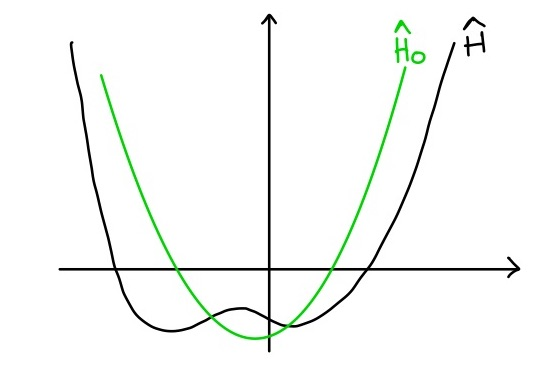
\includegraphics[scale=0.20]{img_1.jpg}
\caption{How to approximate an otherwise very difficult function with a known, simpler one.}
\label{fig:approximation}
\end{figure}
\textbf{1)} First we proceed by writing the S.E. with the truncated basis set.
\[
\hat{H}\bigg(\sum_{m=1}^{M}c_m^{(n)}\psi_m(x)\bigg)=E_n\bigg(\sum_{m=1}^{M}c_m^{(n)}\psi_m(x)\bigg)
\text{ where $c_m^{(n)}=\int dx\,\psi_m^*(x)\varphi_n(x)$}
\]
since the Hamiltonian operator is a function it can be propagated through the equation. Right now we are expanding $n$ and projecting it onto $m$.\\
\[
\sum_{m=1}^{M}c_m^{(n)}\,\hat{H}\psi_m=E_n\,\sum_{m=1}^{M}c_m^{(n)}\psi_m\]
\textbf{2)} We project both functions on the basis (scalar product). We multiply both sides for an arbitrary wave function $\psi_l$ (that we can supposedly solve).
\[\sum_{m=1}^{M}\,(\psi_l,\hat{H}\psi_m)c_m^{(n)}=E_n\,\sum_{m=1}^{M}c_m^{(n)}(\psi_l,\psi_m)
\]
The inner product between two functions gives an integer. \\
$H_{lm}=H_{ml}^*$ is an hermitian matrix that can be diagonalized to get the eigenvalues.\\
\[
\sum_{m}^{M}H_{lm}c_m^{(n)}=E^{(n)}c_l
\]
We reduced a complex problem to a conventional eigenvalue problem with a $H_{lm}$ matrix. The pain is to compute the $M$ integrals and to find an appropriate "problem B". As a results, this method is hardly applicable to any problems with more of 3 dimensions. \\

\section{Quantum tunneling - The Landau problem}
\begin{figure}[htbp!]
	\centering
	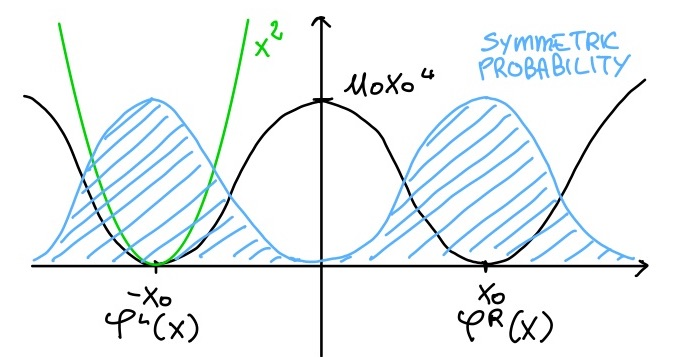
\includegraphics[scale=0.30]{img_2.jpg}
	\label{fig:ass}
	\caption{ass problem}
\end{figure}
The ass problem (because the potential kinda looks like an ass) is the gate to the understanding of quantum tunneling (necessary for quantum bonds, which are a reflection of the quantum tunneling behaviour). \\
The potential is: $U(x)=U_0(x^2-x_0^2)^2$.\\

The Hamiltonian for the wave function: $\hat{H}=-\frac{\hbar^2}{2m}\,\frac{d^2}{dx^2}+U_0\cdot(x^2-x_0^2)^2$
Note that this is a symmetric function, roughly composed by two gaussians, so we can approximate the function with an harmonic oscillator. Considering the potential to its lowest points it can be approximated and then expanded. \\

We have two basis elements, the two eigenstates $n=0,1$ (ground state and first excited state), and we wish to solve $\hat{H}\varphi_n=E_n\varphi_n$, with $n=0,1$:

\[
\hat{H}\varphi_n=E_n\varphi_n
\begin{cases}
\varphi_0 \cong C_L^0\,\psi^L(x)+C_R^0\,\psi^R(x)\\
\varphi_1 \cong C_L^1\,\psi^L(x)+C_R^1\,\psi^R(x).
\end{cases}
\]
$C_L$ and $C_R$ are coefficients for each part of the function, one for each eigenstate. The values $\varphi_o$ and $\varphi_1$ are the two eigenvalues of a $2 \times 2 $ matrix.\\
We then proceed to calculate the value of the matrices for the expansion.\\
\[
H_{RR}=(\psi_R,\hat{H}\,\psi_R)= \int\psi_R^*(x)\,\bigg[-\frac{\hbar^2}{2m}\,\frac{d^2}{dx^2}+U_0\cdot(x^2-x_0^2)^2\bigg]\,\psi_R(x)\,dx\]
\[
=\int\psi_R^*(x)\,\bigg[-\frac{\hbar^2}{2m}\,\frac{d^2}{dx^2}+\frac{1}{2}m\omega^2\cdot(x^2-x_0^2)^2\bigg]\,\psi_R(x)\,dx
\]
$U_0$ has been substitued with the potential energy of the harmonic oscillator approximation. The integral is computable with Taylor expansion because we consider the minimum of the function.
\[
U(x)=U(x_0)+U'(x_0)(x-x_0)+\frac{1}{2}\,U''(x_0)(x-x_0)^2+\dots\]
The final result is
\[
H_{RR}=\frac{1}{2}\hbar\omega
\]
and since this is a symmetrical problem we can also foresee that $H_{LL}\cong\frac{1}{2}\hbar\omega$.\\
The result of $H_{LR}=H_{RL}$ is expected to be very small because the probability of finding the particle in the middle of the harmonic oscillator is very small, i.e. when $\psi_L(x)$ is large, $\psi_R(x)$ is going o be small and viceversa.
\[
H_{RL}=H_{LR}=\int dx\,\psi_L(x)\hat{H}\psi_R(x) = \varepsilon
\]
Now we can calculate the matrix
\[
H_{mn}=
\begin{pmatrix}
E_0 & -\varepsilon\\
-\varepsilon & E_0
\end{pmatrix}
=
\begin{pmatrix}
\frac{1}{2}\hbar\omega & -\varepsilon\\
-\varepsilon & \frac{1}{2}\hbar\omega
\end{pmatrix}
=
E_0
\begin{pmatrix}
1 & -\frac{\varepsilon}{E_0}\\
-\frac{\varepsilon}{E_0} & 1
\end{pmatrix}
\]
\textbf{NB:} $E_0>>>\varepsilon$ because of the energy barrier due to $H_{mn}$.
\newline
We reduced a complex problem to a linear algebra problem: $\hat{H}\psi=E\psi \rightarrow H_{mn}C_n^{(l)}=E_lC_n^{(l)}$.\\
\newline
\textbf{Ansatz 1}: In the ground state I have 50\% probability of finding the particle
\[
\text{G.s.:}
\begin{pmatrix}
1 & -\frac{\varepsilon}{E_0}\\
-\frac{\varepsilon}{E_0} & 1
\end{pmatrix}
\begin{pmatrix}
1\\1
\end{pmatrix}
=
\frac{1}{\sqrt{2}}
\begin{pmatrix}
1-\frac{\varepsilon}{E_0}\\1-\frac{\varepsilon}{E_0}
\end{pmatrix}
\]
This ground state has slightly lower energy than the normal ground state
\[
\text{$1^{st}$ ex. st.:}
\begin{pmatrix}
1 & -\frac{\varepsilon}{E_0}\\
-\frac{\varepsilon}{E_0} & 1
\end{pmatrix}
\begin{pmatrix}
1\\-1
\end{pmatrix}
=
\biggl(1+\frac{\varepsilon}{E_0}\biggr)\cdot E_0 \cdot
\begin{pmatrix}
1\\-1
\end{pmatrix}
\]
\textbf{NB:} If the barrier is infinite the ground state is trivially degenerate. I then have two independent quantum systems. The particle cannot change its state. Instead, if the barrier is finite (slightly determined end of the barrier at very high energies) it splits into two states (\textbf{splitting states}) that interact with each other. The particle goes back to a 100\% probability of being in either one or another system. This is called \textbf{quantum superposition}.
\newline
Since the barrier is at very high energy, we could expect to find the correspondance principle at some point. Classical interpretation of the system at this point says that the particle could "decay" from a state of very high energy into one of the two ground states (50\% probability for each state, fair game). Quantum interpretation gives the 100\% probability to the electron of being in both the states at the same time.\\
\[
\begin{cases}
\varphi_0(x) = \frac{1}{\sqrt{2}}[\psi^L(x)+C_R^0\,\psi^R(x)]\\
\varphi_1(x) = \frac{1}{\sqrt{2}}[\psi^L(x)+C_R^0\,\psi^R(x)]
\end{cases}
\]
\newline
So, if at $t=0$, the  particle is on the left $\ket{\psi_0}=\ket{\psi_L}$, the function immediately after will be $\psi_L(x)$. However, if we wait long enough, the probability to find it in each state will be 50\% - 50\%. \\
What is the probability of finding the particle on the right at given time $t$? \\
$(P_R(t>0)=\,?$)\\
$P_L(t>0)=1-P_R(t>0)$\\
By definition $E_0=0, E_1= \varepsilon$. Consequently, $\varepsilon = E_1-E_0$\\
To find the probability of the particle being on the right/left, ($P_{R/L}(t)=|\braket{\psi_{R/L}\,|\,\varphi(t)}|^2$), we will use the time evolution operator.\\
\[
P_R(t)=|\mel{\psi_R}{e^{-\frac{i}{\hbar}\cdot t \hat{H}}}{\psi_L}|^2
\]
Minding that $\psi_R$ occurs at time $t$ whilst $\psi_L$ occurs at $t=0$.\\
If I want to check whether the particle is still on the left
\[
P_L(t)=|\mel{\psi_L}{e^{-\frac{i}{\hbar}\cdot t \hat{H}}}{\psi_L}|^2
\]
Let's first compute the probability for a small $t$. We perform the Taylor expansion of $e^{-\frac{i}{\hbar}\cdot t \hat{H}} = \mathds{1} -\frac{i}{\hbar}\cdot t\hat{H}$
\[
\ket{\psi_L}=\begin{pmatrix}
1\\0
\end{pmatrix}
\text{, }
\ket{\psi_R}=
\begin{pmatrix}
0\\1
\end{pmatrix}
\text{, }
\hat{H}=
\begin{pmatrix}
0 & \varepsilon\\ \varepsilon & 0
\end{pmatrix}
\]
\[
P_R(t)\cong\bigg|\mel{\psi_R}{\mathds{1}-\frac{i}{\hbar}\cdot t \hat{H}}{\psi_L}\bigg|^2 \cong
\bigg|(0,\,1) \bigg[\mathds{1}-\frac{i}{\hbar}\cdot t\hat{H}
\begin{pmatrix}1\\0\end{pmatrix}\bigg]\bigg|^2
\]
\[
\cong \frac{t^2}{\hbar^2}\varepsilon^2
\]
but since $\frac{t\varepsilon}{\hbar}<<1$ we get $t << \frac{\hbar}{\varepsilon}$.\\
This is telling us that by waiting a little time the probability of finding the particle on the other side increases. This phenomenom is called \textbf{quantum tunneling}.\\
The conclusion up until this point is
\begin{itemize}
	\item A quantistic particle can cross an energy barrier, and the probability (or 		rate at which the transitions happen) is given by
	\[
	k=\frac{\varepsilon}{\hbar}
	\]
	which is an exponentially small amount.\\
	There is an analogy between thermal kinetic activation and quantum tunneling, both 	happen because of stochastic fluctuations. ($K\propto e^{\frac{\Delta V}{K_B T}}$)		. The difference is that in a quantum system this happens in quantum time and is 		not influenced by the temperature of the system.\\
	\item In quantum tunneling, the superposition between the higher energy levels 			that is caused by the lowering of the potential barrier causes the splitting of 		the lower energy levels. This is remarkably important when considering the 				\textbf{formation of the hydrogen bond $\rightarrow$ electron sharing is quantum 		tunneling!}\\
	At infinite distance we don't have any sharing because it's like having an 				infinite energy barrier. When the two atoms get close to each other, they share an 	electron via quantum tunneling, because of this then the energy levels split and 		create the two orbitals (bonding, antibonding).\\
\end{itemize}

For the final $t$ we cannot expand the exponent like we did before. Given $e^{-\frac{it}{\hbar}\hat{H}}\ket{\psi_R}$, we don't know $H\psi_R$, but can rewrite $\psi_R$ as linear combination of eigenstates of $H$:
\[
\text{ground state:} \ket{0}=\bigg(\frac{\ket{L}+\ket{R}}{\sqrt{2}}\bigg) \rightarrow \sqrt{2}\ket{0}= \ket{L}+\ket{R}
\]
\[
\text{first excited state:} \ket{1}=\bigg(\frac{\ket{L}-\ket{R}}{\sqrt{2}}\bigg) \rightarrow \sqrt{2}\ket{1}= \ket{L}-\ket{R}
\]
By summing and subtracting,
\[
\begin{cases}
\ket{L}=\frac{1}{\sqrt{2}}(\ket{0}+\ket{1})\\
\ket{R}=\frac{1}{\sqrt{2}}(\ket{0}-\ket{1})
\end{cases}
\]
so we can substitute them and use hamiltonian operator:
\[
e^{-\frac{it}{\hbar}\hat{H}}\ket{R}=\frac{e^{-\frac{it}{\hbar}\hat{H}}}{\sqrt{2}}\cdot (\ket{0}-\ket{1})=\frac{1}{\sqrt{2}}\ket{0}-\frac{e^{-\frac{it}{\hbar}\varepsilon}}{\sqrt{2}}\ket{1}
\]
where $e^{-\frac{it}{\hbar}\varepsilon}$ is the relative weight of quantum superposition for the first excited state ($E_1=\varepsilon$). Ground state has an eigenvalue $E_0=0$ as stated above.\\
Let's calculate the probability for the particle to be on the left.\\
\[
P_L=|\braket{L}{\psi(t)}|^2=\bigg|\braket{L}{\bigg(\frac{1}{\sqrt{2}}\ket{0}-\frac{1}{\sqrt{2}}\cdot e^{-\frac{it}{\hbar}\varepsilon} \ket{1} \bigg)}\bigg|^2
\]
Knowing that $\braket{L}{L}=\frac{1}{\sqrt{2}}$ and $\braket{L}{R}=0$,
\[
=\bigg|\braket{L}{\frac{\ket{L}+{R}}{\sqrt{2}}-e^{-\frac{it}{\hbar}\varepsilon}\cdot\frac{\ket{L}-\ket{R}}{\sqrt{2}}}\bigg|^2
=\bigg(\frac{1}{2}-\frac{1}{2}\cdot e^{-\frac{it}{\hbar}\varepsilon}\bigg)^2
=\bigg[\frac{1}{2}-\frac{1}{2}\bigg(\cos\frac{\varepsilon t}{\hbar}+i\sin\frac{\varepsilon t}{\hbar}\bigg)\bigg]^2
\]
\[
P_L=\frac{1}{2}\bigg(1-\cos^2\frac{\varepsilon}{\hbar}t\bigg)
\]
For $t=0$, $P=0$ then $\cos^2x$ grows with a $t^2$ rate.
There is an oscillation (figure \ref{fig:pulsation}) with a given period $T=\frac{\hbar}{2\varepsilon}$.\\
\begin{figure}[htbp!]
	\centering
	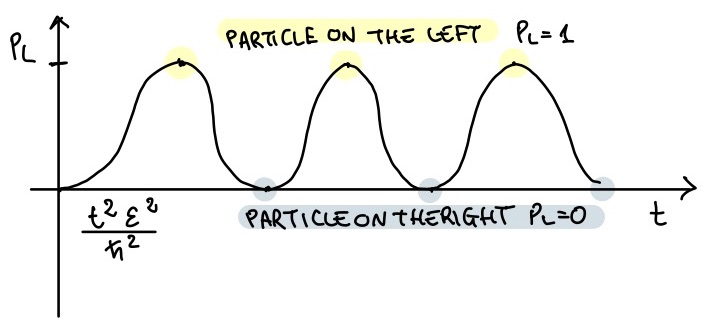
\includegraphics[scale=0.30]{img_3.jpg}

	\caption{The oscillatory behaviour here represented is called \textbf{quantum pulsation}.}
	\label{fig:pulsation}
\end{figure}
\newline

\section{Ritz-Rayleigh variational principle}
Suppose we want to estimate the ground state energy $E_0$ and corresponding wave function of the stationary Schr\"{o}dinger equation.\\
We define $\varphi_n(x)$ as a set of functions approximating $\psi_0(x)$. Variational principle gives an upper bound for the ground state energy. The chosen function's expectation value for energy normally overestimates the g.s. energy; if the chosen function (unfortunately) represent an excited state, the exp. val. of energy for chosen function will highly overcome $E_0$.\\
This set of function is assumed to be complete, so it can always be written as a sum of the linear combination of all the functions:
\[
\varphi(x)=\sum_{n}^{\infty}c_n\psi_n(x),\;\;\; \hat{H}\psi_n=E_n\psi_n\, \text{ furthermore} \;\; \sum_{n=0}|c_n|^2=1
\]
The set of functions is normalized and orthonormal, too. Normalization implies $\sum_{n=0}|c_n|^2=1$.\\
We need to find any function approximating $\psi_0^{(x)}$.\\
The expectation value for $\varphi$ is:
\[
\mel{\varphi}{\hat{H}}{\varphi}=
\braket{\sum_mc_m\psi_m}{sum_nc_n\psi_n}
\sum_{n,m}c_n^{*}c_m\braket{\psi_n\,|\,\hat{H}\,|\,\psi_m}=\sum_{n,m}c_n^{*}c_mE_m\delta_{nm}=
\sum_{n}|c_n|^2E_n=
E_n\sum_n |c_n|^2
\]
We recall that for a normalized set of functions $\sum_{n=0}|c_n|^2=1$ so $\mel{\varphi}{\hat{H}}{\varphi}=E_n$!!! And, of course, by assuming $c_n \geq 0$, the whole operation is $\geq E_0$ but this is true only if $\psi_n=\psi_0$.\\
\newline
TRIVIAL NOTE: if $\varphi(x)=\psi_0$ then we have a projection on a vector on itself:
\[
\begin{cases}
c_n=0, & n \neq 0\\
c_n=1, & n=0
\end{cases}
\]
\newline
The point here is that if we guess a function, compute the eigenvalues, and do the same with another function, the one that lowers the energy the most is the most accurate approximation of the wavefunction.
E.g.:\\
Function 1 $\rightarrow$ Expected value $E_0$\\
Function 2 $\rightarrow$ Expected value $E_1$\\
$\rightarrow$ if $E_0 < E_1$ then $E_0$ is a better approximation of the wave function.\\
\newline
\noindent\rule{4cm}{0.1pt}
\newline
\textit{Example: Given $\varphi(x, \alpha)$, which is a family of wave functions, find $\psi_0(x)$ such as it is the best approximation of the family.} In other words, we need to evaluate the following equation\\
\[
\braket{\varphi_{\alpha}(x)\,|\,\hat{H}\,|\,\varphi_{\alpha}(x)}=E(\alpha)
\]
for whih $E$ is minimum.
We must find the minimum of the function (derivative = 0).
\[
\frac{\partial}{\partial\alpha}E(\alpha)=0\, \text{  solve for  }\, \alpha=\alpha_{min}
\]
Find $\alpha$ such as $E_{\alpha min}$ is the best approximation of $E_0$ and $\varphi_{\alpha min}(x)$ is the best approximation of $\psi_0$.
Putting it formally, if we have multiple parameters: $\varphi_{\alpha \dots \alpha_n(x)}$
\[
\braket{\varphi_{\alpha \dots \alpha_n(x)}\,|\,\hat{H}\,|\,\varphi_{\alpha \dots \alpha_n(x)}} = E_{\alpha \dots \alpha_n}
\]
We need to calculate the minimum of the multidimensional function:
\[
\nabla_{\alpha}E=0 \rightarrow
\begin{cases}
\frac{\partial}{\partial \alpha_1}=0 \rightarrow \alpha_1=\alpha_{1, min}\\
\dots\\
\frac{\partial}{\partial \alpha_n}=0 \rightarrow \alpha_n= \alpha_{n, min}\\
\end{cases}
\]
Doing so we find a collection of energies and wavefunctions.
The more parameters we have, the more we can explore the space, but  we have no guarantee of finding the exact solution.
Indeed, the probability of getting the right ground state is very low.
\newline
\noindent\rule{4cm}{0.1pt}
\newline
\\
So which are the steps of this approximation method? Let's go through them using the quantum harmonic oscillator.\\

Given the Hamiltonian equation for harmonic oscillator: $\hat{H}=-\frac{\hbar^2}{2m}\frac{d^2}{dx^2}+\frac{1}{2}m\omega^2x^2=\braket{T}+\braket{U}$\\
1) \textbf{Variational Ansatz}: We "guess" a normalized (the $4$ term is used for normalization) gaussian to best represent the harmonic oscillator: $\varphi_{\alpha}(x)=\bigg(\frac{1}{\sqrt{2\pi}\alpha}\bigg)^{1/2}e^{-{\frac{x^2}{4\alpha^2}}}$\\

2) \textbf{Computation of $E(\alpha)$} by first evaluating the hamiltonian function of $\varphi_{\alpha}(x)$ (first fragment, so to say)
\[
-\frac{\hbar^2}{2m}\frac{d^2}{dx^2}\varphi_{\alpha}(x)=
\]
\[
=\,\frac{\hbar^2}{2m}\bigg(\frac{1}{\sqrt{2\pi}\alpha}\bigg)^{1/2}\frac{d}{dx}e^{-{\frac{x^2}{4\alpha^2}}}
\]
\[
=\,\frac{\hbar^2}{2m}\bigg(\frac{1}{\sqrt{2\pi}\alpha}\bigg)^{1/2}\cdot\frac{d}{dx}\frac{x}{2\alpha^2}e^{-{\frac{x^2}{4\alpha^2}}}
\]
\[
=\,\frac{\hbar^2}{2m}\bigg(\frac{1}{\sqrt{2\pi}\alpha}\bigg)^{1/2}\cdot\bigg(\frac{1}{2\alpha^2}e^{-{\frac{x^2}{4\alpha^2}}}-\frac{x^2}{2\alpha^2}e^{-\frac{x^2}{4\alpha^2}}\bigg)
\]
\[
=\,\frac{\hbar^2}{2m}\bigg(\frac{1}{\sqrt{2\pi}\alpha}\bigg)^{1/2}\cdot\frac{1}{2\alpha^2}\cdot\bigg(1-\frac{x}{2\alpha^2}\bigg)e^{-{\frac{x^2}{4\alpha^2}}}
\]
The total kinetic energy for this approximation of the quantum oscillator is:
\[
\braket{T}=\frac{\hbar^2}{4m\alpha^2}\bigg[1-\frac{x^2}{2\alpha^2}\bigg]e^{-{\frac{x^2}{4\alpha^2}}}\cdot\frac{1}{(\sqrt{2\pi}\alpha)^{1/2}}
\]
And go on with the evaluation of $E(\alpha)$.
\[
E(\alpha)=\frac{1}{\sqrt{2\pi}\alpha}\cdot \int dx\, e^{\frac{x^2}{2\alpha^2}}\bigg[\frac{\hbar^2}{4m\alpha^2}\bigg(1-\frac{x^2}{2\alpha^2}\bigg)+\frac{1}{2}m\omega^2x^2\bigg]=
\]
\[
=\frac{1}{\sqrt{2\pi}\alpha}-\bigg(\frac{\hbar^2}{8m\alpha^4}+\frac{1}{2}m\omega^2\bigg)\cdot \int\,dx\,\frac{e^{\frac{x^2}{2\alpha^2}}}{\sqrt{2\pi}\alpha}x^2
\]
The integrand is called \textbf{gaussian variance} and it is equal to $\mathbf{\alpha^2}$.
So
\[
E(\alpha)=\bigg(\frac{1}{4}-\frac{1}{8}\bigg)\frac{\hbar^2}{m\alpha^2}+\frac{\alpha^2}{2}m\omega^2 = \frac{1}{8}\frac{\hbar^2}{m\alpha^2}+\frac{\alpha^2}{2}m\omega^2
\]
The latter sum is a sum of two energy values.
\begin{figure}[htbp!]
	\centering
	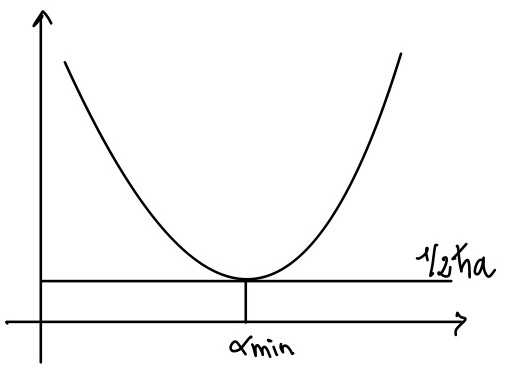
\includegraphics[scale=0.20]{img_4.jpg}
	\caption{In this picture we can see a point of intersection because we get the exact result.}
	\label{fig:intersect}
\end{figure}
To find $\alpha_{min}\rightarrow\frac{\partial}{\partial \alpha}E(\alpha)=0$
\[
\frac{\partial}{\partial \alpha}E(\alpha)=-2\cdot\frac{1}{8}\frac{\hbar}{m\alpha^{3}}+\alpha m\omega^2=0
\]
Multiply by $\alpha^3$ both sides:
\[
\frac{\partial}{\partial \alpha}E(\alpha)=-\frac{\hbar}{4m}+\alpha^4m\omega^2=0
\]
\[
\alpha^2=\sqrt{\frac{\hbar^2}{4m^2\omega^2}}
\]
This is the same result we got for the quantum harmonic oscillation problem! Keep in mind that this method \underline{only} applies to the ground state.
